\secnumbersection{MARCO CONCEPTUAL}

\subsection{TELESCOPIO VLT}
El VLT, sigla para “Very Large Telescope”, es un telescopio ubicado en el Cerro Paranal a 2635 metros de altura, como parte de la “European Southern Observatory” (o conocida por su sigla ESO). 
Los fines bajo los cuáles se construyó el VLT corresponden a los siguientes \cite{eso1998vlt}:
\begin{itemize}

    \item El mayor área de colecta posible, según los recursos disponibles.
    \item La mayor cobertura de longitud de onda, con tal de explotar completamente todas las ventanas atmosféricas.
    \item Máxima flexibilidad y amplia diversificación instrumental, permitiendo múltiples usos de las instalaciones, incluyendo observaciones simultáneas de múltiples longitudes de onda.
    \item Capacidad limitada por la difracción de la mayor línea de base posible.
    \item Optimización de los procedimientos de operaciones científicas, con tal de permitir la explotación, completa y en tiempo real, de la calidad astronómica del sitio y garantizar un máximo retorno científico.

\end{itemize}

El VLT se compone de una red de 4 telescopios principales idénticos, denominados como “Unitary Telescopes” (o por sus siglas UT), 4 telescopios auxiliares, denominados como “Auxiliary Telescopes” (o por sus siglas AT), Interferómetro (por sus siglas en inglés VLTI) y dos telescopios de survey (por sus siglas en inglés VISTA y VST).

Cada UT posee un espejo principal (denominado M1) de forma cóncava con 8,2 metros de diámetro, instalado en un montura de 22 metros de largo, 10 metros de ancho y 20 metros de alto, como se aprecia en la Imágen \ref{fig:real_mount}. Dicha montura permite al espejo moverse según azimut (eje horizontal) y altitud (eje vertical) \cite{eso1998vlt}, como se muestra en la Imagen \ref{fig:front_ut}, con el azimut como líneas celestes en vertical y la altitud como líneas celestes en horizontal.

\begin{figure}[h]
\centering
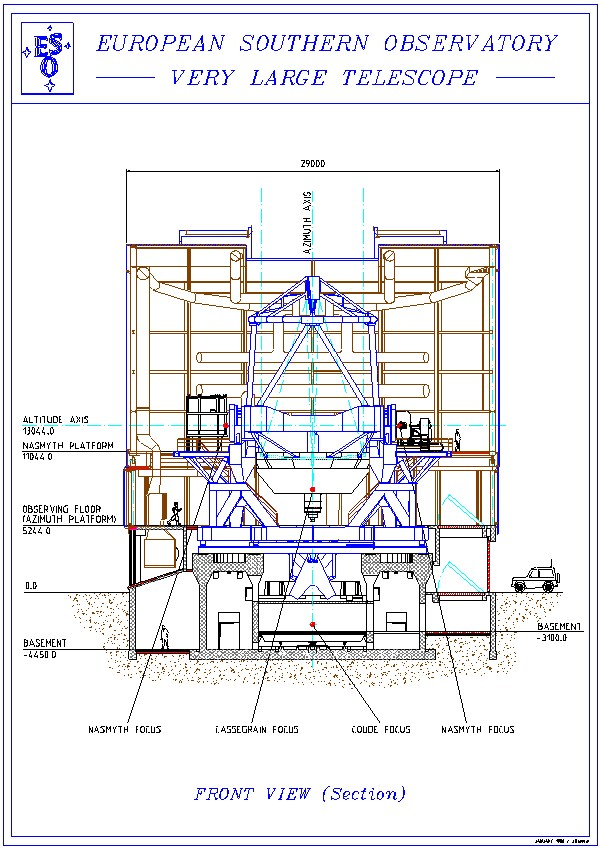
\includegraphics[width=6cm]{figures/front_ut.jpg}
\caption{\label{fig:front_ut} Diagrama frontal de un UT} Fuente: The VLT White Book \cite{eso1998vlt}
\end{figure}

\begin{figure}[h]
\centering
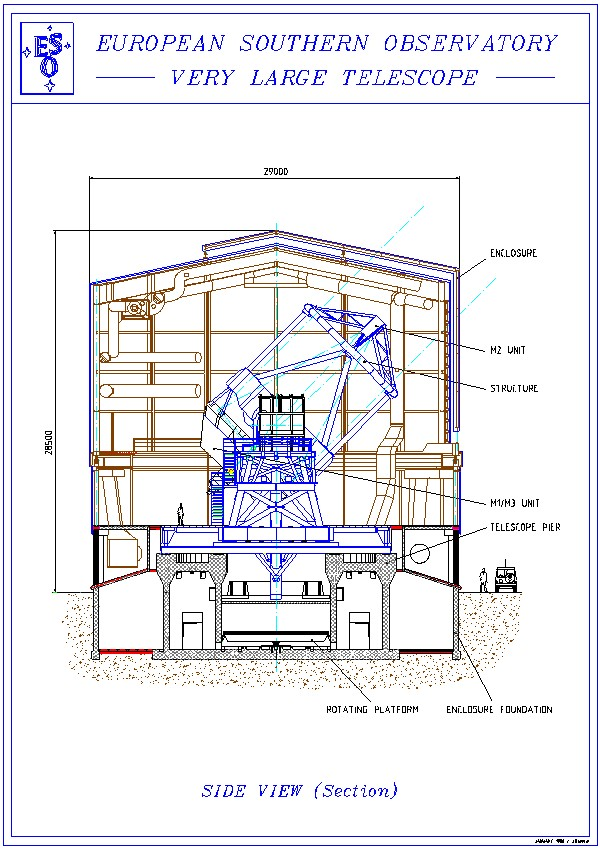
\includegraphics[width=6cm]{figures/side_ut.jpg}
\caption{\label{fig:side_ut} Diagrama lateral de un UT} Fuente: The VLT White Book \cite{eso1998vlt}
\end{figure}

\begin{figure}[h]
\centering
\includegraphics[width=8cm]{figures/real_ut.jpg}
\caption{\label{fig:real_ut} UT 2 visto desde el exterior} Fuente: Elaboración propia
\end{figure}

\begin{figure}[h]
\centering
\includegraphics[width=8cm]{figures/real_mount.jpg}
\caption{\label{fig:real_mount} Montura del M1} Fuente: Elaboración propia
\end{figure}

El M1 está compuesto de espejos más pequeñas, distribuidas en forma de dona. Bajo M1, repartidos en 6 anillos concéntricos, se encuentran 150 actuadores de fuerza axiales; estos son, pistones hidráulicos y neumáticos, donde cada actuador se encuentra debajo de una espejo pequeña respectiva. Estos actuadores dan a M1 una determinada forma óptica, determinada por el patrón de fuerza presentado por los actuadores \cite{eso1998vlt}. El M1 es visible en la Imágen \ref{fig:real_m1}.

\begin{figure}[h]
\centering
\includegraphics[width=8cm]{figures/real_m1.jpg}
\caption{\label{fig:real_m1} Espejo M1, con M2 reflejado y M3 en el centro} Fuente: Elaboración propia
\end{figure}

El M2 consiste de una espejo de 0.9 metros de diámetro, montada a una distancia de aproximadamente 12.3 metros de M1 a lo largo del eje azimutal, con la espejo de M2 apuntando hacia M1. El M2 además está montado sobre un mecanismo electromecánico que sujeta y controla su inclinación \cite{eso2011m2}. El M2 es visible en la Imágen \ref{fig:real_m2}.

\begin{figure}[h]
\centering
\includegraphics[width=8cm]{figures/real_m2.jpg}
\caption{\label{fig:real_m2} Espejo M2} Fuente: Elaboración propia
\end{figure}

El M3 consiste de una espejo elíptica de 1.24 metros de diámetro mayor con 0.86 metros de diámetro menor. Este se ubica dentro de una torre, posicionada en el orificio central del M1. Este puede rotar alrededor de su eje azimutal \cite{eso2011m1}. El M3 es visible en la Imágen \ref{fig:real_m3}.

\begin{figure}[h]
\centering
\includegraphics[width=8cm]{figures/real_m3.jpg}
\caption{\label{fig:real_m3} Espejo M3} Fuente: Elaboración propia
\end{figure}

\subsection{SISTEMA DE ÓPTICA ACTIVA}
La Óptica Activa es un sistema integrado en el M1, encargado de corregir las aberraciones y degradación en la calidad de imágen provocadas por las ópticas del espejo \cite{eso1998vlt}.

Estas aberraciones ópticas suelen ser causadas por la sensibilidad de este a perturbaciones ambientales, cómo las distorsiones térmicas, deformación de espejo por ráfagas de viento, errores de manufactura y mantenimiento del telescopio, entre otros. Esta sensibilidad es causada por la baja proporción entre el grosor y el diámetro del espejo, la cuál es la principal característica que permite al espejo M1 tener su gran tamaño, debido a que esta proporción es la que permite deformar el espejo \cite{wilson1987active}.

El ciclo básico del sistema de Óptica Activa se ilustra en la imágen del Anexo 1. El mismo sigue el siguiente procedimiento:

\begin{enumerate}
    \item El sensor de frente de onda Shack-Hartmann toma una imagen de una estrella en el cielo y la toma como guia\cite{eso1998vlt}.

    \item Se analiza la imágen y se miden las perturbaciones ópticas, calculando las aberraciones\cite{wilson1987active}.

    \item Cuando la desviación es considerable, se genera un set de fuerzas que se deben aplica al M1 para corregir las perturbaciones \cite{wilson1987active}.

    \item Se aplica el set de fuerzas al espejo M1 y, durante una observación, el sensor de frente de onda Shack-Hartmann toma una nueva imágen, repitiendo el proceso\cite{wilson1987active}. Un ejemplo de imágen tomada por el sensor Shack-Hartmann se muestra en la Imágen \ref{fig:sh}.

    \begin{figure}[h]
    \centering
    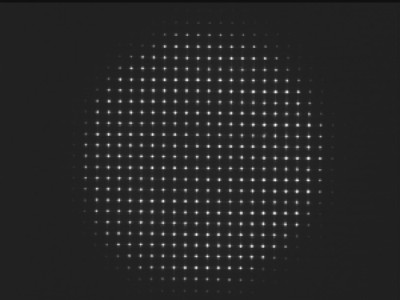
\includegraphics[width=8cm]{figures/sh_eje.png}
    \caption{\label{fig:sh} Imágen capturada por un sensor de frente de onda Shack-Hartmann} Fuente: Implementation of adaptive optics in fluorescent microscopy using wavefront sensing and correction\cite{azucena2010ao}
    \end{figure}

     \item Todo este ciclo es repetido hasta que la imágen tomada durante el Paso 1 venga con una calidad óptica\cite{wilson1987active}.

\end{enumerate}

\subsection{SENSOR DE FRENTE DE ONDA}
Un sensor de frente de onda es un dispositivo electrónico diseñado para calcular las aberraciones ópticas presentes en una imágen tomada, ya sea en el espectro visible o en infrarrojo. El VLT usa CCD Shack-Hartmann como sensores de frente de onda, con cada UT poseyendo uno en un brazo mecánico específico para los sensores.\cite{eso1998vlt}

El objetivo del uso de sensores Shack-Hartmann es la medición de distorsiones del frente de onda capturado desde la fuente, sobre las cuáles se realiza el proceso de Óptica Activa.\cite{eso1998vlt}

\subsection{LOGS}
Logging se refiere al proceso de registrar diferentes eventos y actividades que ocurren dentro de un sistema de software \cite{jayathilake2011mind}. Estos registros suelen almacenarse en archivos para su posterior análisis, tanto por parte de desarrolladores como de operadores externos.

Los registros de log son los únicos tipos de datos que, valga la redundancia, registran información de la operación interna de un sistema de software, por lo que su rol en la industria es importante. Debido a esto mismo, los registros de log pueden alcanzar tamaños en el orden de hasta el orden de millones de líneas\cite{ma2023automatic}.

Los registros de log de los telescopios UT registra un día completo de operación, donde se registra información sobre las condiciones ambientales, el funcionamiento del sistema de Óptica Activa, la toma de imágenes durante periodos de calibración y de observación, entre otros. Debido a lo anterior, estos registros de log suelen alcanzar el orden de cientos de miles de líneas. Un ejemplo de estos registros de log puede verse en el Anexo 2.

Las líneas de un registro de log estan compuestas de tokens estáticos y valores dinámicos. Los tokens estáticos corresponden a cadenas de texto que entregan metadata e información complementaria sobre el dato reportado en las líneas, y como tal se repiten de forma sistemática a lo largo del registro. Los valores dinámicos son cadenas de texto o números que entregan el valor del dato reportado, y por ende no se repiten con un patrón claro en el registro \cite{ma2023automatic}. 

\subsection{ANÁLISIS DE LOGS}
Originalmente, el análisis de registros de logs era realizado por desarrolladores con el fin de trazar el flujo de ejecución del sistema de software, identificar excepciones y potenciales errores. \cite{jayathilake2011mind}

Actualmente este enfoque se ha expandido a casos de uso en otros servicios en la industria \cite{ma2023automatic}, debido a que, por la naturaleza de la información contenida en los registros de log, su análisis permite a los operadores detectar, diagnosticar e incluso predecir errores que puedan afectar la disponibilidad y el rendimiento del sistema de software \cite{jayathilake2011mind}.

En el pasado, durante la prevalencia del enfoque original, el análisis de registros de log era realizado aplicando revisiones visuales y reglas construidas manualmente. Sin embargo, la complejidad de los sistemas de software actuales ha llevado a la complejización de sus respectivos registros de logs, por lo que ya no es posible depender solamente de los métodos anteriormente mencionados. \cite{ma2023automatic}

Por esto, en los últimos años se ha desarrollado ampliamente el área del análisis automatizado de registros de logs, mejorando su eficiencia y exactitud mediante la aplicación de tecnologías distribuidas y técnicas de machine learning. \cite{ma2023automatic}

\subsection{ESTRUCTURACIÓN DE LOGS}
Los registros de logs generalmente poseen una composición demasiado compleja como para ser interpretada de forma directa y manual; sin el acceso de conocimiento profesional, es difícil seleccionar de forma manual las reglas apropiadas para la comprensión de los registros de log \cite{ma2023automatic}. Por esta condición es que se refiere a que los registros de log sean “No Estructurados” o “Semi Estructurados”. 

Además, el gran tamaño de los archivos de log promedio también se vuelve un problema para el análisis manual de los registros de log \cite{ma2023automatic}.

Debido a esto, durante los últimos años, se han desarrollado herramientas, procedimientos y frameworks para el análisis automático de registros de log, y una parte considerable de los esfuerzos realizados se enfocan en la “Estructuración” de los registros de log.

Actualmente, el workflow de análisis automático de registros de log se divide en 2 etapas centrales \cite{ma2023automatic}:

\begin{itemize}
    \item Log Parsing: Se toman los registros semi-estructurados de log y se generan plantillas a partir de estos. Una plantilla es una sentencia estructurada que se repite entre varios registros de log, dividiéndose en los tokens estáticos y valores dinámicos. \cite{ma2023automatic}

    \item Feature Extraction: Se aplican las plantillas generadas sobre los registros de log para obtener las características, esto es, las variables dinámicas, de los mismos. \cite{ma2023automatic}

\end{itemize}

\subsection{ORIGENES DE DATOS}

Tres origenes de datos son considerados para la presente memoria:

\begin{enumerate}
    \item Registros de log: El origen de dato más importante para esta memoria, considerando la problemática a resolver. Estos datos son propios de los telescopios UT, y como tales, se obtienen directamente de los mismos una vez terminada su ejecución \cite{eso1998vlt}

    \item Imágenes en formáto fits: Las imágenes tomadas por el telescopio usan el formato fits, el cuál es universal en ciencias y astronomía\cite{nasa2025fits}. Es formato se divide en dos secciones: el contenido científico y el Header, donde este último contiene la metadata que describe a la misma imágen que lo aloja, como por ejemplo su número de ID, su tiempo de exposición, las fechas de inicio y término de grabado, entre otros\cite{nasa2025fits}. Para el caso de esta memoria, solo importan las imágenes que fueron tomadas desde el sensor de frente de onda como parte del ciclo de Óptica Activa.


    \item Observaciones en formáto csv: La ESO mantiene en una página web con el fin de archivar la información sobre todas las observaciones válidas de los UTs. Desde esa página se pueden obtener los datos de todas las observaciones de un día mediante una query. La información disponible en la página puede incluir el número de ID de la observación, la fecha de inicio, el tiempo de exposición, el instrumento de captura de la imágen, entre otros.

\end{enumerate}